\chapter{Mejora de la aplicación}\label{cap:mejoras}

Para la realización de este proyecto fin de carrera se decidió buscar herramientas que hicieran uso de tarjetas gráficas para comprobar contraseñas. Tras una búsqueda exhaustiva se determina que la aplicación \emph{Distributed Hash Cracker} era la más completa y, lo más importante, la única que disponía de una licencia abierta que nos permitía poder realizar cambios sobre ella.

Como ya se mencionó en la introducción, el uso de software libre es muy importante para la seguridad por el hecho de que al disponer del código fuente se pueden realizar auditorías sobre el mismo. Además, en caso de que la empresa que desarrolla el software dejase de darle soporte siempre cabría la posibilidad de que otra empresa pudiera ofrecer dicho soporte. Por otra parte, el software libre no solo tiene ventajas en la seguridad, sino que ofrece la garantía de que si la empresa deja de desarrollar dicho software, o ésta desapareciese, siempre quedaría el software a disposición del público pudiendo tomar otro el relevo sobre el mantenimiento, sin que puedan realizarse acciones legales contra éste por infracción de derechos de autor. En este punto se debe mencionar que hay que obedecer siempre los términos de la licencia del software y, en especial, el Real Decreto Legislativo 1/1996, de 12 de abril, por el que se aprueba el Texto Refundido de la Ley de Propiedad Intelectual, que es la ley que regula los derechos de autor en España.

\emph{Distributed Hash Cracker}, en adelante DHC, es un software que permite determinar la palabra utilizada en una función resumen para devolver un determinado resumen. Para ello hace uso de un sistema de fuerza bruta~\cite{dhc:paper}. Éste software se encontraba alojado en la página \url{http://rpisec.net/}, pero por cuestiones desconocidas ha desaparecido dejando de tener soporte. Esto nos ha animado a realizar las modificaciones que necesitábamos para conseguir una aplicación completa y, especialmente, más fácil de mantener y que permitiera añadir funcionalidades de forma sencilla.

DHC es un software que se distribuía bajo licencia BSD\footnote{La licencia libre BSD permite realizar modificaciones sobre el software siempre y cuando se mantenga la mención de autoría en el mismo, pero no obliga a distribuir el código en caso de dar copias de la aplicación.}. Esta herramienta está programada en C++, ensamblador y PHP y es capaz de distribuir el trabajo entre un conjunto de máquinas, denominadas agentes. Los agentes se encargan de procesar tareas criptográficas tanto en CPU como en GPU dependiendo de los algoritmos implementados en cada caso.

Aunque DHC es una muy buena herramienta tiene algunas deficiencias que hacen que necesite modificaciones en algunos puntos importantes de su código para garantizar que la herramienta pueda sobrevivir en el futuro.

El mayor problema actualmente es que aún estando escrito en un lenguaje orientado a objetos, no se hace uso de las características del mismo cuando se debería. Por ejemplo, el código de las funciones resumen de que dispone está entremezclado. Esto supone un gran problema al implementar nuevas funciones resumen, ya que implica tener que ver qué partes de código se deben adaptar y cuáles no. Por tanto, es necesario hacer un cambio de cómo controla DHC estas funciones de tal modo que sea más sencillo el mantenimiento de la herramienta.

Por otra parte, la implementación de funciones resumen de que dispone DHC, aún estando relativamente bien surtida, creemos que podría ser necesario en un futuro la implementación de más funciones resumen u otro tipo de comprobaciones sobre seguridad (como pudiera ser redes WiFi). Esto significa que hay que realizar los cambios necesarios que permitan en un futuro añadir funcionalidades diferentes a las inicialmente planteadas sin que esto suponga un esfuerzo demasiado elevado.

Finalmente, DHC dispone de un programa que se encarga de controlar el reparto de las tareas. Este programa se denomina controlador y está desarrollado enteramente en PHP sin seguir un modelo claro de organización del código. En un principio parece que está basado en el patrón arquitectónico MVC, pero por algún motivo el código fuente parece muy entremezclado.

\section{Lenguajes de programación utilizados}

El lenguaje de programación elegido para el proyecto ha sido C++. Esta elección se realiza por diversos factores:

\begin{itemize}
	\item Tanto los lenguajes C como C++ son completamente compatibles con CUDA. Además, CUDA ofrece algunas ayudas específicas para C++ (como la forma de definir texturas) facilitando el trabajo con dicha tecnología. Éste tipo de ayudas es más patente cuando se utiliza el método sencillo de desarrollo.
	
	\item El autor del presente proyecto final de carrera está muy familiarizado con dicho lenguaje lo que permite realizar mejor el desarrollo.
	
	\item Aunque no hace un uso adecuado de las capacidades de C++, DHC ha sido desarrollado utilizando dicho lenguaje de programación.
\end{itemize}

Por otra parte se hace uso del lenguaje PHP para el controlador web por ser un lenguaje gratuito y muy extendido. Además, dispone de versiones para Windows, Linux y MacOS X.

Por último se hace uso de una variación del lenguaje C creada por NVIDIA para desarrollar en sus tarjetas gráficas. Esta variación consiste en añadir información sobre el acceso a métodos y variables:

\begin{itemize}
	\item Se usa \_\_global\_\_ para denotar funciones que se alojarán en la tarjeta gráfica, pero que podrán ser llamadas desde la CPU.

	\item \_\_device\_\_ son funciones que solo pueden ser llamadas desde otras funciones que ya se encuentren en la GPU.
	
	\item Las variables que pueden ser compartidas entre distintos \emph{threads} se denotan con \_\_shared\_\_. Estas variables hacen uso de la memoria global.
	
	\item Si se necesitase que una función resida en la CPU se le indicaría con \_\_host\_\_.
	
	\item Si utilizamos memoria que no pueda cambiar de valor dentro de la GPU utilizaremos la notación \_\_constant\_\_ y deberemos iniciar la memoria desde la CPU.
\end{itemize}

En caso de necesitar más detalles sobre la arquitectura CUDA en~\cite{nvidia:cuda_c_programming_guide} se puede encontrar una guía completa sobre las peculiaridades de la implementación de C realizada por NVIDIA.

\section{Estudio de DHC}

DHC es una aplicación divida en dos partes claramente diferenciadas y que es importante comprender de cara a poder realizar modificaciones de forma satisfactorias sobre el. Estas partes son el controlador y el agente.

\subsection{Controlador de DHC}
El controlador es la herramienta encargada de gestionar las tareas solicitadas, permitir al usuario la introducción de tareas y la cancelación de las mismas, realizar estadísticas de uso, etc. A continuación se expone de manera más detallada las tareas realizadas por el controlador:

\begin{itemize}
	\item Introducción de nuevos resúmenes a probar. Estos resúmenes son almacenados en una base de datos para garantizar la persistencia de la tareas y así, en caso de caída, poder recuperar el trabajo.

	\item Crear paquetes de claves a probar y repartirlos entre los agentes para comprobar un determinado resumen. Estos paquetes son denominados unidades de trabajo (WU en sus siglas en inglés y que será la nomenclatura utilizada en este documento). Una WU es una estructura que contiene la información de la tarea a realizar. Esta información contiene datos como:

	\begin{itemize}
		\item Tipo de algoritmo que se desea utilizar, como pueden ser MD5, SHA-1, etc.
	
		\item Datos sobre los que realizar las comprobaciones. En el caso de las funciones resumen este dato se corresponde con el hash que queremos comprobar.
	
		\item Juego de caracteres a utilizar. Permite elegir si utilizar número y letras minúsculas o mayúsculas. También permite seleccionar símbolos, espacio y retorno de carro.
	
		\item Longitud máxima esperada. Ésta se utiliza para restringir las pruebas, ya que consideramos que una cotraseña no va a exceder de los 8 caracteres no es necesario probar más allá.
	
		\item Bloque de claves a comprobar. Esto es el conjunto de contraseñas que se van a probar indicadas por su posición inicial (el primer valor a probar) y final.
	\end{itemize}
	
	\item Mide los tiempos transcurridos desde que un controlador recibe una WU hasta que devuelve un resultado, calcula la velocidad de ejecución en hash/s y muestra informes de velocidad y carga de trabajo del sistema.
	
	\item Controlar los tiempos de expiración de las tareas y las prioridades de las mismas.
\end{itemize}

De este modo el controlador es una de las partes más importantes del sistema al ser la interfaz que el usuario va a utilizar para utilizar los recursos del mismo.

El controlador hace uso de una base de datos MySQL, conocida por ofrecer un buen rendimiento y por ser software libre. Gracias al uso de esta base de datos la aplicación consigue de forma sencilla garantizar la persistencia de los datos en caso de caídas del sistema. Hay que recordar que sólo hay un controlador y en caso de que éste deje de estar activo todo el sistema se viene abajo, por lo que es importante garantizar que la información con la que éste trabaja no se pierda.

Cada vez que una WU es dada a un agente, se calcula un tiempo de vida que será el tiempo que tiene el agente para devolver un resultado antes de considerar que esa WU ha caducado. Si una WU caduca será reciclada y ofrecida a otro agente.

El controlador esta programado enteramente en PHP sin hacer uso de ningún \emph{framework} sino que haciendo uso del patrón arquitectónico MVC se ha programado desde cero todo el sistema. Al no disponer de documentación se hace relativamente complejo realizar el mantenimiento de esta solución, especialmente cuando no siempre hace uso del patrón anteriormente mencionado.

\subsection{Agente de DHC}

El agente es el encargado de realizar la tarea más compleja del sistema que es la comprobación de los resúmenes dados por el controlador utilizando para ello las herramientas que estén a su disposición (la CPU y si puede ser la GPU).

El agente se encuentra en el equipo que va a realizar las operaciones de comprobación de funciones resúmenes y puede haber tantos equipos como se necesite. De este modo el sistema no está restringido a un único agente y puede distribuir la carga de trabajo entre tantos agentes como haga falta. Además, los agentes no tienen porque estar restringidos sólo a una red local, también pueden distribuirse a lo largo de internet, de modo se podría tener varias sedes que ejecuten agentes disponiendo de un único controlador. En caso de requerir un sistema más complejo se puede consultar el apartado~\ref{sec:conf_avanzada}.

Por otro lado, cuando se ejecuta un agente sobre un ordenador, éste realiza una comprobación del número de CPUs en el sistema y del número de GPUs con capacidad para utilizar CUDA. Lo que se pretende con esto es crear un proceso ligero encargado de cada unidad de cómputo que haya en el sistema, teniendo en cuenta que para cada GPU asigna una CPU. Esto significa que si disponemos de un sistema con 4 GPU y 8 CPUs (concretamente 8 núcleos) sólo considerará que hay 4 GPUs y 4 CPUs (las otras 4 CPUs las utiliza para control de las unidades de tarjeta gráfica).

A grandes rasgos, el proceso de ejecución de un agente, tras haberse configurado es el mostrado en la figura~\ref{fig:cont_proc_ejec}. Los apartados más importantes de este proceso son la obtención de la WU y la ejecución de la misma.

\begin{figure}
	\centering
	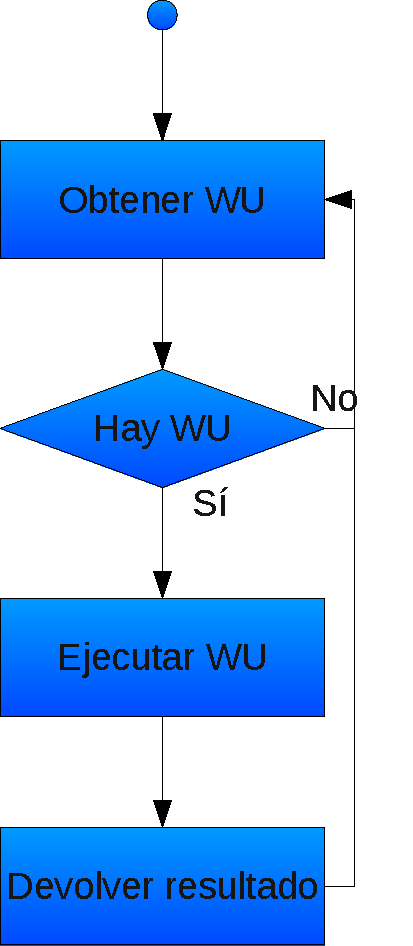
\includegraphics[width=0.26\textwidth]{images/proc_cont.pdf}
	\caption{Proceso de ejecución de un controlador}\label{fig:cont_proc_ejec}
\end{figure}

Durante el proceso de obtención de una WU, el agente comprueba si esta es valida para el algoritmo indicado. Para ello utiliza el siguiente código:

\begin{lstlisting}[language=c]
if(algorithm == "md4" || 
  algorithm == "md4_fast" || 
  algorithm == "md5" ||
  algorithm == "md5crypt" ||
  algorithm == "ntlm")
{
  hashlen = 16;
}
else if(algorithm == "sha1")
  hashlen = 20;
else        
  ThrowCustomError("Unknown hash function");
                
if(algorithm != "md5crypt" && hashlen*2 != text.length())
  ThrowError("Invalid hash length");

//Sanity check
if(hashlen > 256)
  ThrowError("Hash length too long");
if(text.length() == 0)
  ThrowError("Empty hash");
\end{lstlisting}

El problema del código mostrado anteriormente es que requiere forzosamente ser modificado ante cualquier cambio de un algoritmo, o ante la creación de un algoritmo nuevo. De este modo el código no aprovecha la capacidad de abstracción que otorga el lenguaje C++, ya que podría haberse hecho esto de un modo más elegante como se comprobará más adelante. Además, el código mostrado supone un problema para el mantenimiento ya que éste se encuentra en un fichero del código fuente, pero además, en otro completamente distinto también se hacen comprobaciones sobre los algoritmos por lo que hay que tener un buen conocimiento sobre la estructura interna de los ficheros del programa.

\section{Modificaciones realizadas a DHC}

Como se ha podido ver en el apartado anterior DHC es una buena aplicación, pero tiene algunos fallos que podrían resolverse para mejorar la mantenibilidad de la solución. Esto ofrecería una mayor esperanza de vida al programa y lo convertiría en una herramienta mucho más útil a corto y largo plazo.

Por los motivos anteriores se ha decidido realizar los cambios necesarios que conviertan a DHC en una herramienta más fácil de manejar, de mantener y que permita a cualquier programador añadir funcionalidades de forma sencilla sin requerir un alto grado de conocimiento del código del agente.

\subsection{Diseño de API para algoritmos de codificación}\label{sec:api_alg}

Como se ha comentado anteriormente, una de las mayores deficiencias de DHC, a nuestro entender, es la falta de un mecanismo sencillo para incorporar nuevos algoritmos debido, principalmente, a que el código de los algoritmos se entremezcla con la funcionalidad del controlador en distintos ficheros de código fuente. Esto supone un problema importante, a la hora de realizar nuevos algoritmos, al encontrarse todo el código de los mismos repartido entre distintas funciones y métodos, dificultando enormemente las labores de mantenimiento y de desarrollo. Por este motivo se ha decidido implementar una API para facilitar el desarrollo de algoritmos, que aprovechando todas las funcionalidades ya existentes, mejore de forma sustancial las labores de mantenimiento de la aplicación.

El diseño de la API propuesta se ha basado en dos ideas:
\begin{itemize}
	\item El algoritmo como sistema para la realización de una tarea específica, como pueda ser obtener el valor que generó un determinado resumen y
	
	\item La factoría, que es el mecanismo que permite acceder a los algoritmos que existan en el sistema.
\end{itemize}

El objetivo principal de la propuesta es permitir agrupar todo el código que rige a un algoritmo de forma que facilite la modificación del mismo y, en caso necesario, crear algoritmos nuevos sin tener que realizar un gran esfuerzo.

Gracias al API propuesto, cada algoritmo será una clase que herede de \emph{Algorithm}. Esta clase abstracta define las funcionalidades mínimas que debe implementar un algoritmo para poder ser utilizado por el agente. Así se consigue englobar en un único lugar todo lo relativo a un algoritmo.

La clase \emph{Algorithm} define los siguiente métodos obligatorios de implementar:

\begin{description}
	\item[GetName] Devuelve el nombre del algoritmo. Este nombre se utiliza para poder identificar el algoritmo y poder seleccionarlo cuando se solicite. Para garantizar el buen funcionamiento del sistema y evitar funcionamientos extraños, este nombre debe ser único.
	
	\item[HashLength] Es el tamaño que debe tener un hash para ser considerado válido. Con esto se pretende que en caso de que el controlador nos de un hash erróneo poder hacer frente al problema.

	\item[InputLength] Tamaño de la entrada recibida por el WU. Aunque en muchos casos solo comprobando el tamaño del hash sería suficiente, hay algoritmos que pueden necesitar entradas extendidas, por lo que se necesita un doble chequeo.

	\item[ExecuteCPU] Implementa el código que se encarga de utilizar la CPU para realizar la tarea solicitada.

	\item[ExecuteGPU] Ejecuta en una GPU el algoritmo con objeto de realizar la tarea de comprobación.
	
	\item[IsGPUCapable] Indica si el algoritmo tiene soporte de GPU. De este modo el sistema sabe si puede determinar el método por el que debe realizarse el procesamiento, si por CPU o por GPU.
	
	\item[IsCPUCapable] Indica si el algoritmo soporta procesamiento utilizando CPU.
\end{description}

Por otra parte se ha creado una factoría de algoritmos (la clase \emph{AlgorithmFactory}) que permite acceder de forma sencilla a los algoritmos que se encuentren registrados en el sistema. Además, esta factoría permite el registro de nuevos algoritmos de forma sencilla para facilitar la implementación de nuevas utilidades.

Para poder comprender mejor como funciona el nuevo sistema la figura~\ref{fig:algotirmo_gpu} muestra a grandes rasgos como sería el proceso. En este caso el actor es el agente que va a hacer uso de la funcionalidad ofrecida para realizar una comprobación sobre MD5.

\begin{figure}
	\centering
	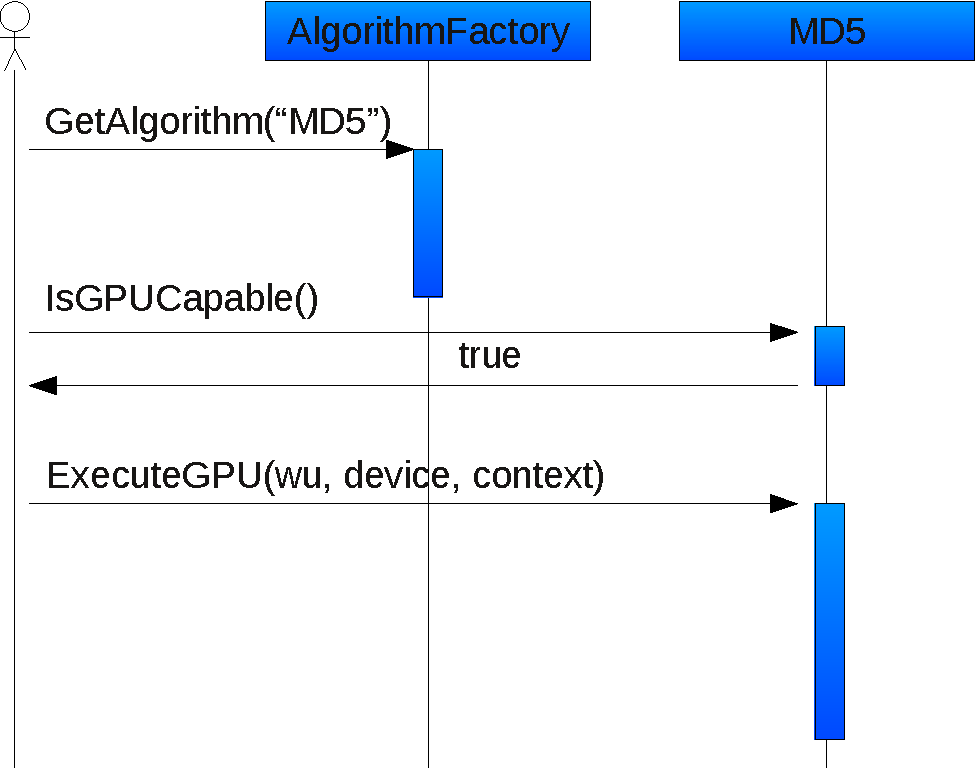
\includegraphics[width=0.7\textwidth]{images/algoritmo_gpu.pdf}
	\caption{Diagrama de secuencia de la ejecución de un algoritmo en GPU}\label{fig:algotirmo_gpu}
\end{figure}

A la hora de implementar estas características hay que tener en cuenta que se puede hacer uso tanto de una CPU como de una GPU. Esto supone que el algoritmo debe estar capacitado para ofrecer alguna de dichas opciones y, a poder ser, ambas. Esto supone en la práctica que tanto el algoritmo implementado puede esta duplicado disponiendo del código de la versión de CPU y de la versión de GPU.



\subsection{Diseño de API para la estandarización de la ejecución de algoritmos}

Una vez creado el API para algoritmos se puede comprobar que muchos algoritmos siempre siguen el mismo patrón de ejecución. Esto supone tener que repetir constantemente el mismo código en los algoritmos cuando podríamos hacer uso de la reutilización para eliminar este inconveniente. Por este motivo se planteó diseñar un sistema que permitiera estandarizar la forma que tiene un algoritmo de ejecutarse de tal modo que sólo tengamos que centrarnos en lo imprescindible de cada uno de ellos.

La filosofía que se ha empleado es la misma que en el caso de los algoritmos. En este caso se ha creado la clase \emph{Executor} que se encarga de definir las funcionalidades básicas que debe implementar un mecanismo de ejecución y por otro lado se dispone de la clase \emph{ExecutorFactory} que nos facilita el acceso a los mismos.

Con este sistema se obtiene un mecanismo muy interesante para la realización de pruebas de algoritmos sin tener que modificar el resto de algoritmos y, en caso de obtener un mecanismo suficientemente bueno y que pueda ser utilizado por más algoritmos, de organizar todos los algoritmos que deban ejecutarse de igual forma para reducir la cantidad de código duplicado facilitando el mantenimiento en caso de errores.

El código original de DHC utiliza el mismo mecanismo de ejecución para todos los algoritmos implementados. Esto está muy bien hasta cierto punto ya que restringe de forma muy clara la cantidad de mecanismos que pueden implementarse en el sistema. Gracias a la nueva API se permite implementar más algoritmos, no teniendo que restringirnos necesariamente a una forma concreta de hacer las cosas o a un tipo concreto de algoritmos (hasta el momento solo hay funciones resumen).

\begin{figure}
	\centering
	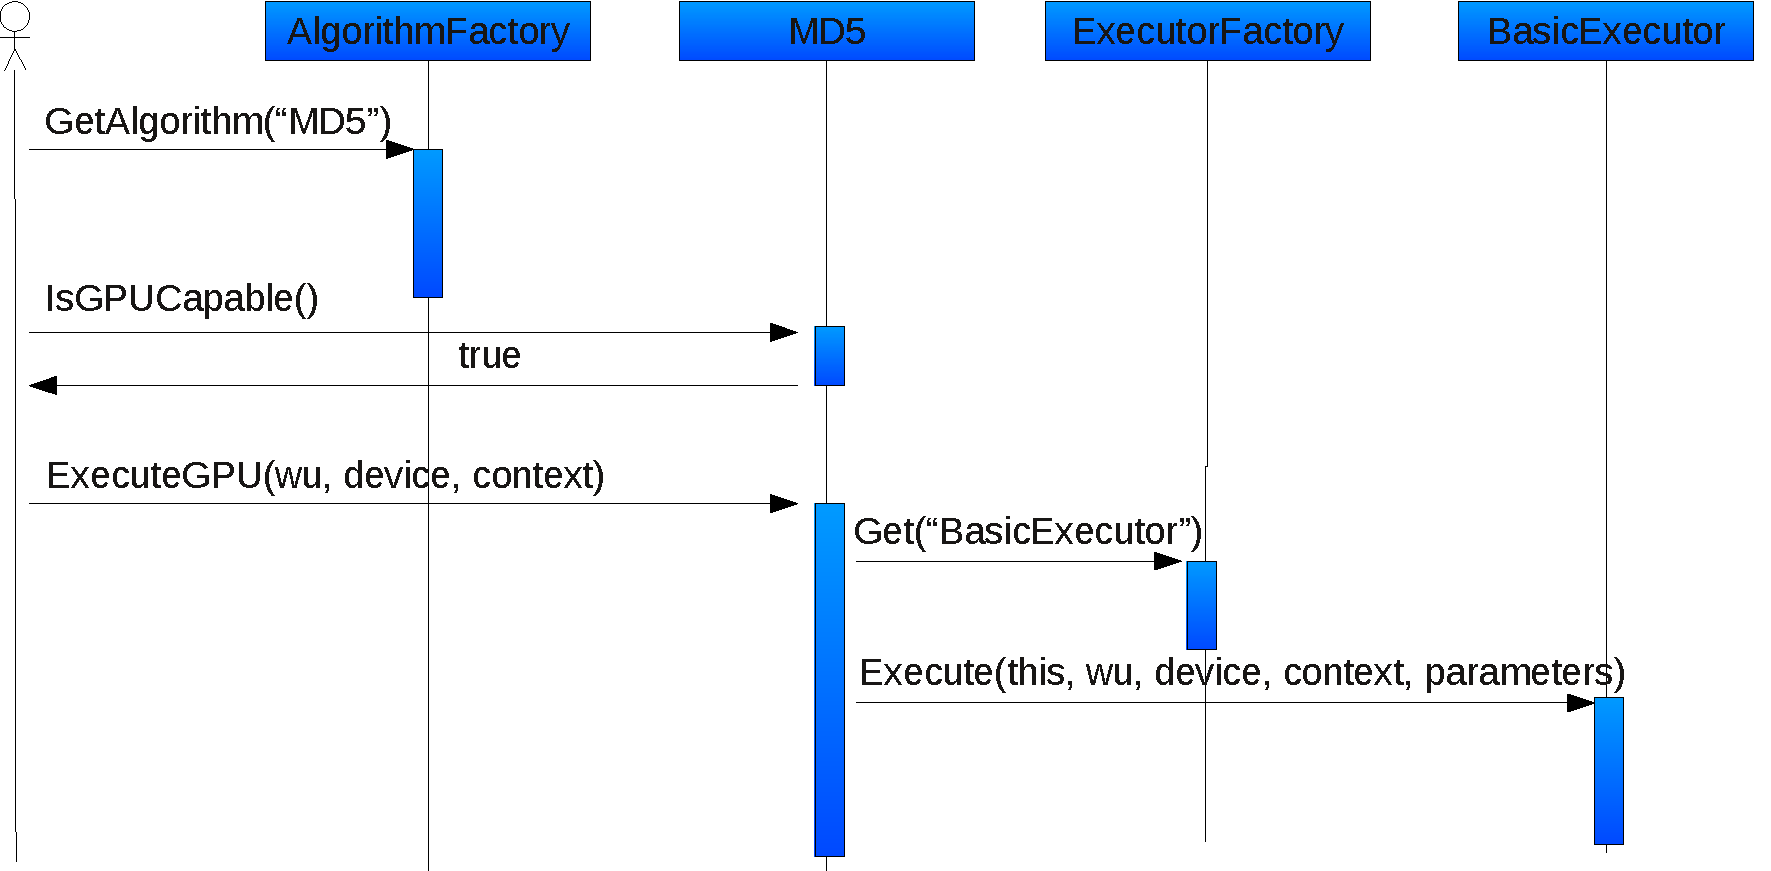
\includegraphics[width=1\textwidth]{images/executor.pdf}
	\caption{Diagrama de secuencia de la ejecución de un algoritmo en GPU utilizando un \emph {Executor}}\label{fig:algotirmo_gpu_executor}
\end{figure}

La ejecución con este mecanismo se complica un poco más (ver figura~\ref{fig:algotirmo_gpu_executor}), pero la sobrecarga introducida por este mecanismo es despreciable en tiempo. Además, hay que tener en cuenta que no es obligatorio el uso de un \emph{Executor} por parte de un algoritmo.

Una de las principales ventajas que podemos comentar sobre este sistema es que ahora un algoritmo no tiene porque estar sujeto a un único modo de hacer las cosas. Se puede detectar si hay un \emph{Executor} en concreto y si no está se pude seleccionar otro. Así, en caso de que se retire uno por cuestiones de mantenimiento o depuración el sistema podría seguir funcionando (siempre que se implemente esta forma de trabajar).

Por otra parte se permite, gracias a la arquitectura utilizada, la creación de \emph{proxys}, objetos intermedios que capturan la funcionalidad expuesta para realizar operaciones de forma transparente. Por ejemplo, se podría disponer de un \emph{proxy} para los algoritmos que permitiese hacer un seguimiento de las llamadas ejecutadas en caso de que el algoritmo no tuviese habilitada la generación de trazas de ejecución.

En la figura~\ref{fig:alg_ex_prox} puede verse como pueden interactuar entre sí los distintos elementos expuestos en este apartado. Como puede comprobarse, la versatilidad del nuevo sistema permite gran cantidad de configuraciones que pueden ser utilizadas siempre que sea necesario. Para comprender mejor la gráfica, los círculos representan algoritmos, las cajas son \emph{Executors} y las flechas son asociaciones de uso. Por ejemplo, \emph{MD5} usa \emph{BasicExecutor}.

\begin{figure}
	\centering
	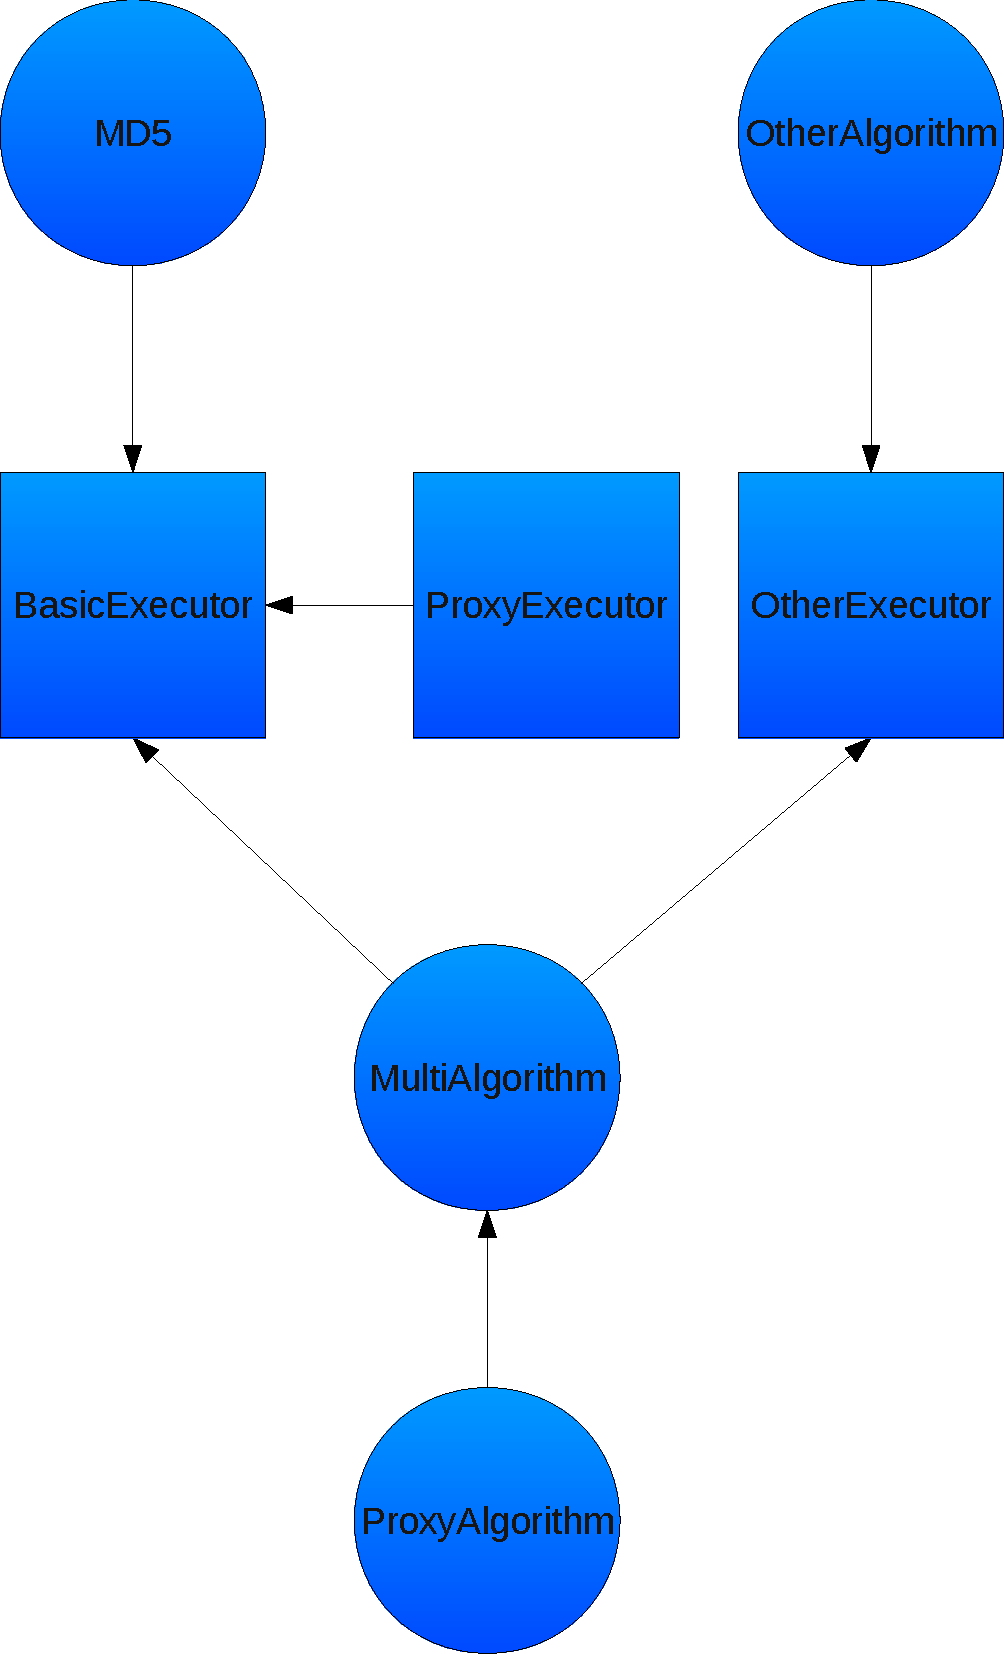
\includegraphics[width=0.4\textwidth]{images/algorithms_executors_proxys.pdf}
	\caption{Panorámica de uso de \emph{Algorithms} y \emph{Executors}}\label{fig:alg_ex_prox}
\end{figure}

\subsection{Modificaciones para la mejora de la escalabilidad}

Durante las primeras pruebas realizadas sobre DHC se notó que el tiempo de respuesta de la interfaz web podía verse seriamente afectado si la velocidad utilizada por los agentes para solicitar tareas o devolver tareas es muy alta y si la distancia entre el agente y el controlador es grande. Este último punto se constató cuando se hicieron pruebas en las que el controlador se encontraba en un servidor en Alemania y el agente se encontraba en España. Sin duda la ralentización en este punto se debía a las latencias de la red por la espera de los asentimientos (paquetes ACK de la arquitectura IP). Estos retrasos pueden afectar de forma importante en la escalabilidad del sistema, por lo que se ha decidido realizar cambios para eliminar en la medida de lo posible estos problemas.

Cada agente de DHC se encuentra en un bucle en el que en cada iteración solicita una WU al controlador. En caso de que no haya ninguna tarea que pueda realizar, el agente procede a esperar 5 segundos. Este tiempo puede resultar insuficiente si el controlador tiene que hacer gran cantidad de cálculos o si el número de agentes es tal que saturen con peticiones al controlador (efecto DDoS). Por este motivo se ha diseñado un algoritmo que ajuste el tiempo de espera de forma dinámica para adaptarse mejor a las capacidades del controlador.

El nuevo algoritmo tiene en cuenta el tiempo que tarda el controlador en dar una respuesta al agente y si la respuesta dada contiene o no una WU. Con esto se pretende que el sistema se ajuste mejor a las condiciones ambientales del sistema.

\subsubsection{Control del tiempo con respecto al tiempo de respuesta del controlador}

Siempre que se solicitan WU a un controlador el agente mide los tiempos que tarda en recibir la respuesta. Este tiempo permite controlar si el controlador está empezando a saturarse o no. Así, en caso de que los tiempos empiecen a verse incrementados, y por tanto se considere que el controlador está saturado, se procede a incrementar el tiempo entre solicitudes. Con esto se pretende descargar al controlador de un exceso de carga distribuyéndola en el tiempo.

Por otra parte, en caso de que el tiempo disminuya supondría justo lo contrario, la carga del controlador es menor, por lo que el tiempo de espera puede empezar a reducirse poco a poco. Al realizar una disminución lenta del tiempo de espera se consigue que no se sature de repente el controlador como podría suceder si este tiempo se redujera rápidamente.

\subsubsection{Control del tiempo con respecto a las tareas recibidas}

Aunque el ideal sería que el sistema pudiera estar constantemente funcionando, la realidad dista mucho de esto ya que es fácil que se de el caso de que no haya tareas que procesar o, que habiéndolas, éstas no sean compatibles con los agentes libres.

Teniendo lo anterior en cuenta, es fácil considerar que si en un momento dado no hay tareas, la próxima vez que consultemos al agente éste siga sin disponer de trabajos que asignar. Como este caso puede darse de forma continuada durante muchas consultas creemos que tiene sentido considerar que cada vez que se haga una petición a un controlador, y éste no tenga WUs, la espera hasta la siguiente vez que solicite una tarea se vea incrementado hasta un tiempo máximo. 

En caso de que el controlador empiece a ofrecer de nuevo WU a los agentes, estos empezarán a disminuir el tiempo entre solicitudes de forma paulatina hasta que vuelvan a estar estables.

En la figura~\ref{fig:control_tiempo_espera} puede verse una explicación gráfica de los dos mecanismos explicados. Las variables utilizadas son:
\begin{description}
	\item[Tesp:] representa el tiempo de espera que se utilizará en caso de que se considere que el sistema no está respondiendo correctamente.
	
	\item[Tresp:] contiene el tiempo que ha tardado el controlador en devolver una respuesta al agente.
	
	\item[Tant:] es el tiempo que tardó el agente en responder en la anterior consulta.
	
	\item[MAX\_TESP:] representa el tiempo máximo entre consultas al controlador.
	
	\item[MIN\_TESP:] es el tiempo mínimo entre llamadas al controlador.
\end{description}

\begin{figure}
	\centering
	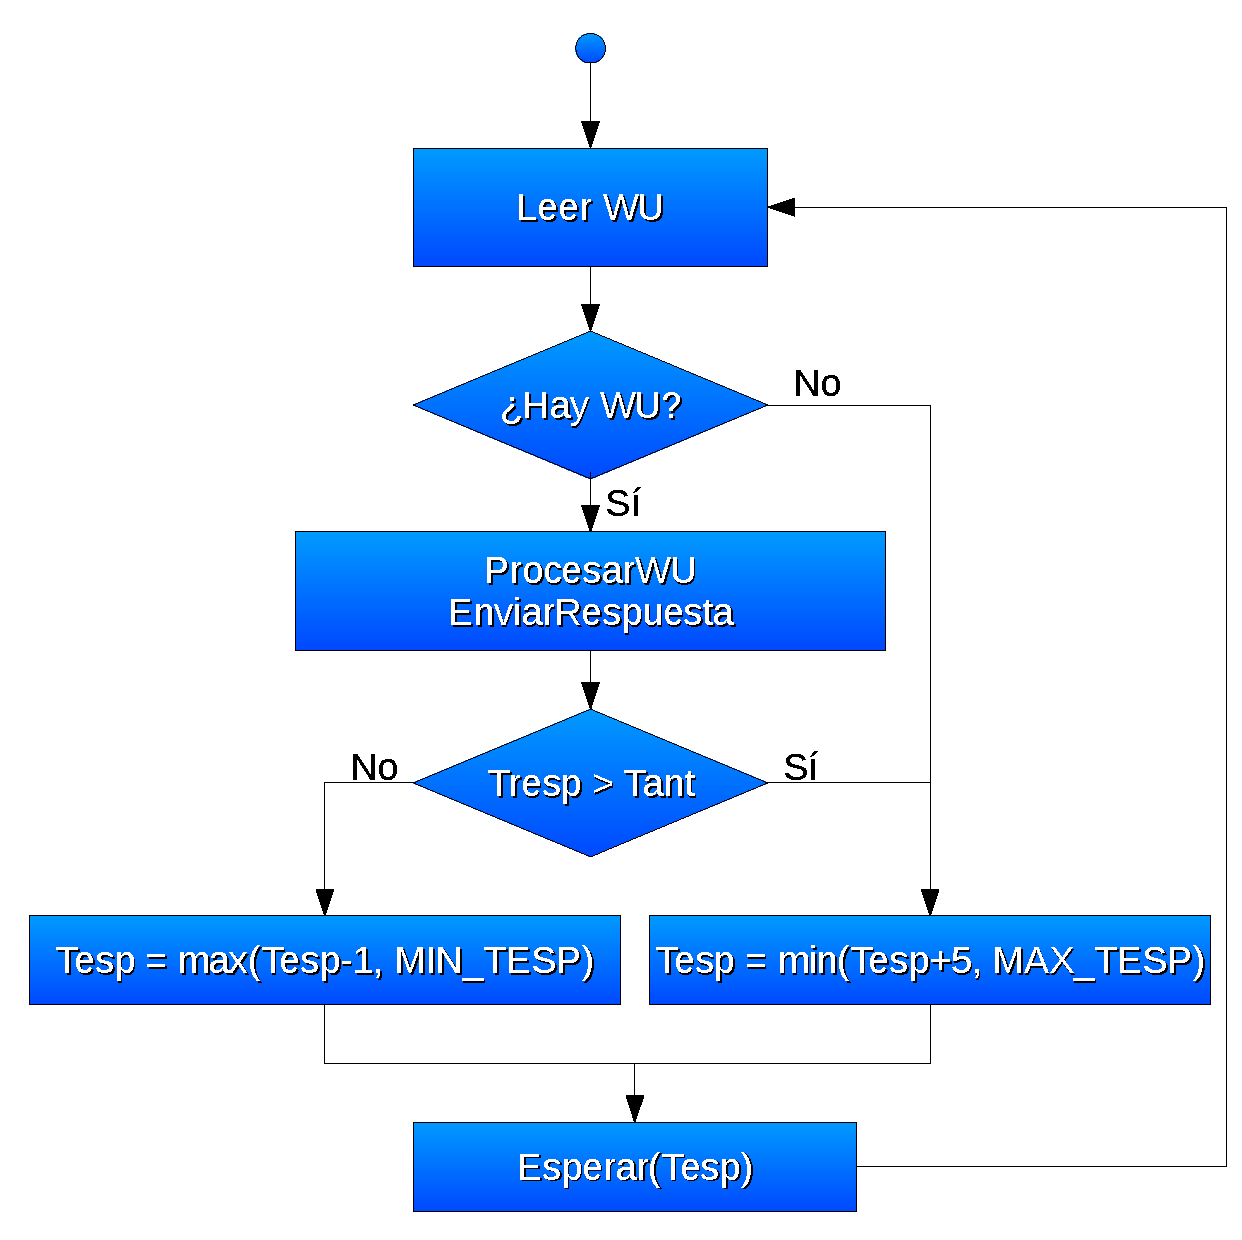
\includegraphics[width=0.7\textwidth]{images/control_tiempo_espera.pdf}
	\caption{Control del tiempo de espera en las solicitudes}\label{fig:control_tiempo_espera}
\end{figure}

\section{Diseño e implementación de un mecanismo de carga de extensiones}

Ahora que se dispone de un API que facilita la creación de algoritmos y mecanismos para ejecutar estos, se ha diseñado un sistema que permite cargar nuevos algoritmos y \emph{Executors} que se encuentren fuera de la aplicación. Estos algoritmos y \emph{Executors} que pueden cargarse de este modo son denominados \emph{plugins}.

Para comprender mejor la idea hay que tener en cuenta que hasta este momento, si se modificaba un algoritmo al estar éste dentro del programa había que generar un nuevo ejecutable con dicha modificación. Lo que se pretende es que el algoritmo no tenga que formar parte del agente y que pueda ser una unidad que se encuentre por separado.

Para poder implementar este apartado se ha desarrollado una serie de clases, (figura~\ref{fig:plugins}) que van a permitir describir el contenido del mismo y añaden facilidades para poder crear instancias de las clases que defina, que se presentan a continuación:

\begin{description}
	\item[PluginFacility:] clase abstracta que describe una funcionalidad que va a presentar el \emph{plugin} al agente. Ésta está identificada por un nombre, su versión y el tipo. Además, permite crear instancias de la funcionalidad.
	
	\item[PluginFacilityAlgorithm:] permite que el \emph{plugin} pueda ofrecer algoritmos a los agentes. Esta clase implementa PluginFacility.
	
	\item[PluginFacilityExecutor:] permite que el \emph{plugin} pueda ofrecer \emph{Executors} a los agentes. Esta clase implementa PluginFacility.
	
	\item[PluginFactory:] esta clase debe ser instanciada en el \emph{plugin} y en ella hay que registrar todos aquellos componentes que ofrecerá el \emph{plugin} al agente. Cada componente a ofrecer deberá heredar de PluginFacility. Además, esta clase proporciona información extra como el autor del \emph{plugin} o el listado de \emph{facilites} que se van a exportar.
\end{description}

Además de lo anterior, los \emph{plugins} deben contener una función llamda \emph{GetPluginFactory} que permitirá obtener la instancia de \emph{PluginFactory} que tiene el \emph{plugin}.

\begin{figure}
	\centering
	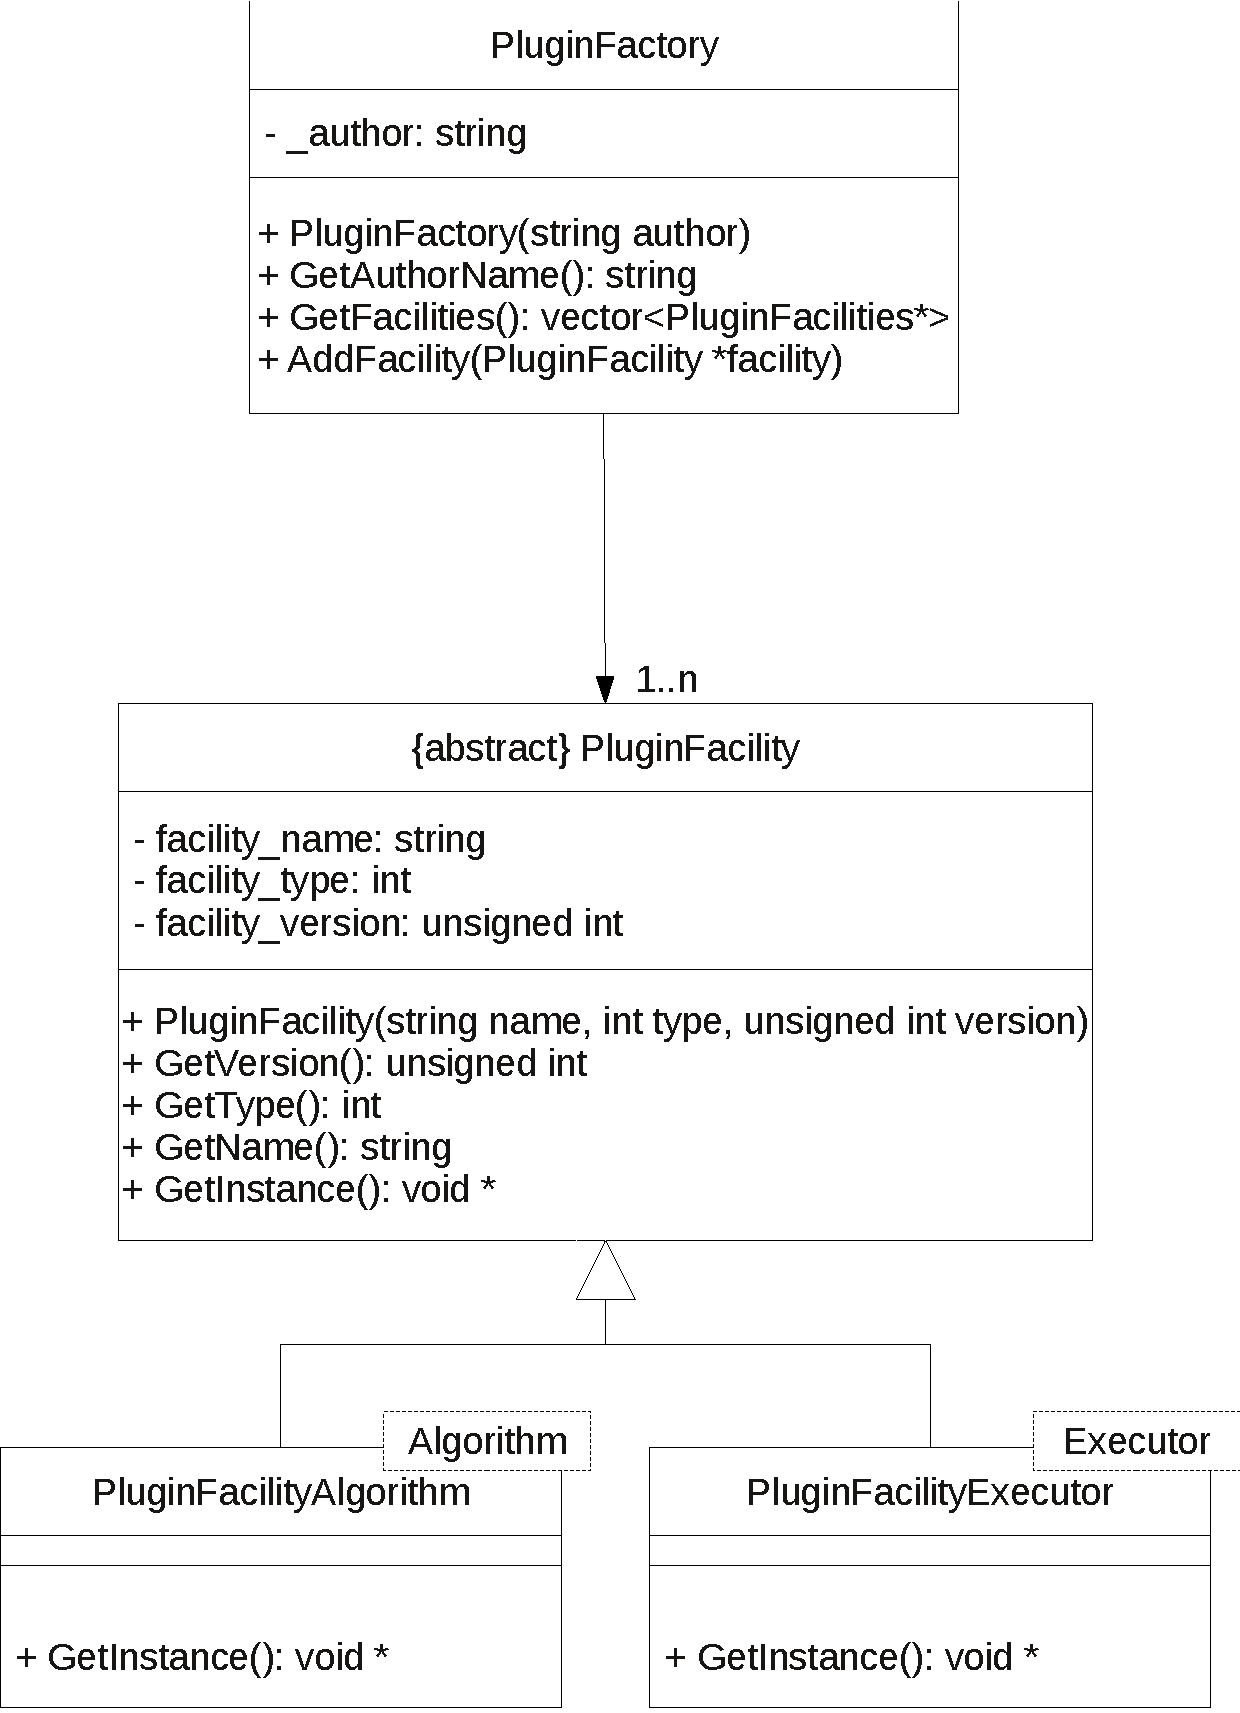
\includegraphics[width=0.7\textwidth]{images/plugins.pdf}
	\caption{Diagrama de clases del sistema de plugins}\label{fig:plugins}
\end{figure}

Como tener que memorizar todo el proceso de crear un \emph{plugin} puede resultar muy complicado (intervienen muchas clases con dependencias entre ellas) se ha añadido una serie de macros de C que permiten simplificar en gran medida la creación de los mismos. Por ejemplo, para la creación del algoritmo que implementa SHA-256 se ha creado una clase denominada sha256 que exportamos como algoritmo del siguiente modo:

\begin{verbatim}
BEGIN_PLUGIN("Samuel Rodriguez Sevilla")
   ADD_ALGORITHM(sha256, "sha256", 1)
END_PLUGIN()
\end{verbatim}

Las macros existentes son:
\begin{description}
	\item[BEGIN\_PLUGIN(author\_name)] Indica que se va a definir un \emph{plugin} y su autor es \emph{author\_name}.
	
	\item[END\_PLUGIN()] Finaliza la definición de un \emph{plugin}.
	
	\item[ADD\_ALGORITHM(class, name, verion)] Añade un algoritmo definido en la clase \emph{class} que será identificado por \emph{name} y cuya versión es \emph{version}.
	
	\item[ADD\_EXECUTOR(class, name, verion)] Igual que el algoritmo, pero para un \emph{Executor}.
\end{description}

\section{Mejoras en la depuración}

Cuando se desarrollan aplicaciones siempre hay que tener muy en cuenta que se pueden producir errores durante la ejecución. Generalmente, el método habitual para comprobar los fallos es utilizar salidas por pantalla tratando de acotar el lugar del fallo; este sistema es poco profesional por lo que para la realización de esta práctica se han utilizado otros mecanismos.

Para comprobar la ejecución de toda aplicación en caso de errores el mejor método es el uso de un depurador, por este motivo se ha utilizado el depurador GNU GDB. Pero aún así no siempre es suficiente con utilizar un buen depurador, sino que tener información extra a la que éste pueda darnos puede ser de gran utilidad. Por este motivo se ha implementado un sistema de trazas para depuración que no buscan la acotación de los errores, esa información ya se encuentra en el fichero de volcado creado en los fallos graves, sino que ofrece una visión más global sobre qué está sucediendo en el código. Esta información puede ser desde cuando se entra en un método, cuando se sale de éste, salida de información varia, etc.

Para activar la salida de depuración se debe llamar a CMake del siguiente modo:
\begin{verbatim}
$ DEBUG=1 cmake .
\end{verbatim}

Así, cuando CMake esté generando el fichero de Makefile tendrá conocimiento de que debe activar la opción de depuración y de generación de salida de depuración. El primero consiste en añadir el parámetro -g durante la compilación y el segundo con -DDEBUG.

Las funciones para utilizar la salida de depuración son:

\begin{description}
	\item[DO\_ENTER(class, method)] Se encarga de anunciar cuándo se entra en un método/función. También configura automáticamente el sistema para controlar cuándo se sale del método/función para que quede constancia. Sus parámetros son cadenas que representan la clase en la que nos encontramos (\emph{class}) y el método (\emph{method}).
	
	\item[DO\_ERROR(str)] Muestra un error por la salida de depuración. Acepta como parámetro la salida que debe mostrar.

	\item[DO\_WARNING(str)] Advierte de una situación extraña, pero que no impide a la aplicación seguir funcionando. Acepta como parámetro la salida que debe mostrar.

	\item[DO\_MESSAGE(str)] Muestra un mensaje de usuario. Acepta como parámetro la salida que debe mostrar.

	\item[DO\_LOG(str)] Muestra un mensaje de seguimiento. Acepta como parámetro la salida que debe mostrar.
	
	\item[DO\_DEBUG(str)] Información de depuración. Es útil cuando se quiere mostrar por la salida de depuración información sobre el estado de ciertas variables. Acepta como parámetro la salida que debe mostrar.

	\item[INIT\_LOG(lvl)] Inicializa el sistema de salida de depuración. Acepta como parámetro el nivel de depuración que se va a utilizar. Este nivel puede ser:
	\begin{description}
		\item[ERROR] Es el nivel más bajo de depuración. Solo se muestran las salidas de error.
		
		\item[WARINING] Siguiente nivel de depuración. Se mostrarán las salidas de los niveles anteriores y las salidas de avisos.
		
		\item[MESSAGE] Muestra las salidas de los niveles anteriores y los mensajes del programador.
		
		\item[LOG] Mensajes de seguimiento y todos los mensajes de los niveles anteriores.

		\item[DEBUG] Mensajes de depuración junto a todos los mensajes de los niveles anteriores.
	\end{description}
\end{description}


\section{Nuevo controlador}

Además de los cambios anteriores realizados al agente también se han realizado cambios en el controlador. Concretamente se ha rehecho completamente reutilizando el código justo. El motivo de la creación de este nuevo controlador se debe, principalmente, a que se quiere disponer de un sistema bien organizado y claramente centrado en la labor de controlar las tareas.

Hasta este momento el controlador se encargaba tanto de administrar las tareas como de codificar los mecanismos necesarios de control para determinar los datos de entrada, las funciones llamadas, etc. Esto se debe principalmente a que no se ha hecho uso de ningún \emph{framework} de desarrollo web que ocultase este tipo de tareas. De este modo el controlador es una aplicación con un código que entremezcla la representación de datos, el control del flujo de ejecución y las tareas administrativas.

Por el motivo anterior se decidió crear un nuevo controlador haciendo uso del \emph{framework} CakePHP (puede encontrarse en \url{http://cakephp.org/}). Este \emph{framework} tiene las siguientes características:

\begin{itemize}
	\item Abstrae la base de datos facilitando el trabajo con los datos independientemente del motor de base de datos utilizado.
	
	\item Maneja el flujo de funcionamiento de la aplicación permitiendo, de este modo, que el programador se centre únicamente en la labor de desarrollo de las funcionalidades del programa.
	
	\item Tiene actualizaciones constantes que, en caso de mejoras de rendimiento o estabilidad, pueden incorporarse fácilmente a nuestro desarrollo sin necesidad de realizar cambios sobre el mismo.
	
	\item Dispone de abundante documentación con gran cantidad de ejemplo, lo que facilita su aprendizaje.
	
	\item Su uso es muy sencillo.
\end{itemize}

Por otra parte, aprovechando este cambio del controlador se ha intentado realizar algunas optimizaciones. Entre ellas podemos destacar:

\begin{itemize}
	\item Optimización de la base de datos. Para ello se estudió el uso que hace el controlador de los accesos y se comprobó que las tablas que se utilizan para realizar las estadísticas son constantemente utilizadas y estas nunca llegan a tener un número de elementos muy elevado (el controlador borra los datos que considera antiguos). Por este motivo se ha decidido pasar estas tablas a la memoria RAM, de modo que el acceso sea más rápido. El mayor problema de esta solución es que en caso de caída de la base de datos se perderían estos valores, pero al no ser información fundamental no supone una gran preocupación.
	
	\item Agrupación de accesos a base de datos. En el antiguo controlador se podía encontrar acciones que realizaban dos o tres accesos a la base de datos para modificar un mismo elemento. Para evitar esta situación lo que se ha hecho ha sido ir acumulando los cambios a realizar y una vez que no se van a hacer más se hace la actualización de la base de datos. Esto permite ahorrar algo de tiempo y reduce la carga sobre la base de datos.
\end{itemize}

Se ha tenido en cuenta el diseño de la web a la hora de reescribir el controlador considerando que un estilo más atractivo ayudaría a una mejor experiencia de usuario.

\section{Algoritmos nuevos de seguridad implementados}

Inicialmente DHC soporta los algoritmos MD4, MD5, SHA1, NTLM y MD5 crypt. Este último es una versión de MD5 utilizada por los sistemas UNIX para almacenar las contraseñas y que se forma de la siguiente forma \$ID\$SALT\$HASH, donde ID es el identificador del algoritmo de resumen empleado (1 para MD5), SALT es una semilla aleatoria que se adjunta a la contraseña a resumir y HASH es el resultado del resumen de la unión de la contraseña y la semilla:

$$HASH = H(SALT | PASSWD)$$

Estos algoritmos se han recodificado para que se adapten a los cambios mencionados en \ref{sec:api_alg}. Tras este cambio se ha procedido al desarrollo de nuevos algoritmos que dotan al sistema de mayor funcionalidad, especialmente si son algoritmos más modernos.

Hay que tener en cuenta que a menos que se hallen debilidades contra los algoritmos el sistema de comprobación a utilizar será siempre el de fuerza bruta. Esto supone que los algoritmos más actuales sean más costosos con respecto al tiempo necesario.

Para el desarrollo de los nuevos algoritmos se ha tenido en cuenta su uso. De este modo no se han implementado aquellos que están en desuso por ser de poca utilidad.

\subsection{SHA-256}

Este algoritmo de resumen busca sustituir al antiguo SHA-1 ya que este se vio seriamente afectado por el tamaño de los resúmenes que generaba (de 128 bits) y por el descubrimiento de ataques controla el mismo (como se ha visto en~\ref{sub:sha1}).

Para codificar este nuevo algoritmo se ha procurado hacer uso de la experiencia previa de la aplicación, procedente del estudio de la misma, y se ha reutilizado parte del código del antiguo SHA-1. De este modo se consigue reducir el tiempo de desarrollo.

La implementación de este algoritmo se ha tomado a partir de la información ofrecida por el NIST~\cite{nist:shs} y se ha probado que funciona correctamente.



